\section{Results and Discussion}

\subsection{GPU Training Performance}

Table~\ref{tab:gpu_training} summarizes the training performance and accuracy metrics for all eight YOLO model variants on the GPU workstation. All models were trained for 300 epochs with early stopping, converging within 150--200 epochs.

\begin{table}[!t]
\caption{GPU Training Performance and Accuracy Metrics}
\label{tab:gpu_training}
\centering
\resizebox{\columnwidth}{!}{
\begin{tabular}{lccccccc}
\toprule
\textbf{Model} & \textbf{mAP@50} & \textbf{mAP@50:95} & \textbf{Precision} & \textbf{Recall} & \textbf{F1} & \textbf{FPS} & \textbf{Training} \\
 & \textbf{(\%)} & \textbf{(\%)} & \textbf{(\%)} & \textbf{(\%)} & & \textbf{(GPU)} & \textbf{Time (h)} \\
\midrule
YOLOv8n & 86.4 & 62.3 & 84.2 & 81.7 & 0.829 & 142.3 & 8.5 \\
YOLOv8s & 89.7 & 67.8 & 87.5 & 85.3 & 0.864 & 98.6 & 17.2 \\
YOLOv10n & 85.8 & 61.5 & 83.6 & 80.9 & 0.822 & 156.7 & 9.1 \\
YOLOv10s & 88.9 & 66.4 & 86.8 & 84.2 & 0.855 & 112.4 & 18.3 \\
YOLOv11n & 87.3 & 63.7 & 85.1 & 82.8 & 0.839 & 148.5 & 8.8 \\
YOLOv11s & 90.2 & 68.9 & 88.2 & 86.1 & 0.871 & 105.3 & 17.8 \\
YOLOv12n & 86.9 & 62.9 & 84.7 & 82.1 & 0.834 & 145.2 & 9.2 \\
YOLOv12s & 89.4 & 67.2 & 87.1 & 84.9 & 0.860 & 101.7 & 18.5 \\
\bottomrule
\end{tabular}
}
\end{table}

\textbf{Key Observations}:

\begin{itemize}
\item \textbf{Small Models Outperform Nano Models}: Across all architectures, small (s) variants consistently achieve 3--4\% higher mAP@50 and 5--6\% higher mAP@50:95 compared to nano (n) variants, demonstrating the expected accuracy-capacity trade-off. YOLOv11s achieves the highest mAP@50 (90.2\%) and mAP@50:95 (68.9\%), followed closely by YOLOv8s (89.7\%, 67.8\%).

\item \textbf{YOLOv11 Shows Consistent Advantages}: YOLOv11 variants demonstrate superior performance compared to other architectures at equivalent model sizes. YOLOv11n achieves 87.3\% mAP@50, outperforming YOLOv8n (86.4\%), YOLOv10n (85.8\%), and YOLOv12n (86.9\%). This advantage is attributed to YOLOv11's refined C3k2 blocks and improved attention mechanisms \cite{4}, \cite{25}.

\item \textbf{YOLOv10 Exhibits Slightly Lower Accuracy}: YOLOv10 variants show marginally lower accuracy (0.6--0.8\% mAP@50) compared to YOLOv8 and YOLOv11, likely due to architectural trade-offs made to enable NMS-free inference. However, YOLOv10 achieves the highest GPU inference speed (156.7 FPS for YOLOv10n), demonstrating its efficiency-oriented design \cite{21}, \cite{33}.

\item \textbf{YOLOv12 Performance}: YOLOv12 variants show competitive but not superior performance compared to YOLOv11, suggesting that recent architectural refinements provide incremental rather than transformative improvements for this specific task \cite{24}, \cite{31}.

\item \textbf{Training Efficiency}: Nano models require approximately 8--9 hours of training, while small models require 17--18 hours, reflecting their increased computational complexity. All models converge reliably without significant overfitting, validating the effectiveness of our data augmentation strategy.
\end{itemize}

\subsection{Raspberry Pi Inference Performance}

Table~\ref{tab:rpi_performance} presents comprehensive inference performance metrics for all models across four optimization formats (PyTorch, ONNX, TFLite, OpenVINO) on Raspberry Pi 4B.

\begin{table*}[!t]
\caption{Raspberry Pi 4B Inference Performance Across Optimization Formats}
\label{tab:rpi_performance}
\centering
\resizebox{\textwidth}{!}{
\begin{tabular}{llcccccc}
\toprule
\textbf{Model} & \textbf{Format} & \textbf{Inference Time} & \textbf{FPS} & \textbf{Model Size} & \textbf{Peak RAM} & \textbf{CPU Usage} & \textbf{mAP@50} \\
 & & \textbf{(ms)} & & \textbf{(MB)} & \textbf{(MB)} & \textbf{(\%)} & \textbf{(\%)} \\
\midrule
\multirow{4}{*}{YOLOv8n} & PyTorch & 142.3 & 7.0 & 6.4 & 512 & 385 & 86.4 \\
 & ONNX & 78.5 & 12.7 & 6.2 & 324 & 378 & 86.2 \\
 & TFLite & 95.2 & 10.5 & 3.1 & 287 & 362 & 84.8 \\
 & OpenVINO & 82.1 & 12.2 & 6.0 & 298 & 371 & 86.1 \\
\midrule
\multirow{4}{*}{YOLOv8s} & PyTorch & 287.4 & 3.5 & 22.4 & 892 & 392 & 89.7 \\
 & ONNX & 156.8 & 6.4 & 21.8 & 567 & 387 & 89.4 \\
 & TFLite & 198.3 & 5.0 & 11.2 & 512 & 375 & 87.9 \\
 & OpenVINO & 163.5 & 6.1 & 21.2 & 541 & 383 & 89.3 \\
\midrule
\multirow{4}{*}{YOLOv10n} & PyTorch & 135.7 & 7.4 & 5.6 & 487 & 381 & 85.8 \\
 & ONNX & 72.3 & 13.8 & 5.4 & 312 & 374 & 85.6 \\
 & TFLite & 89.6 & 11.2 & 2.8 & 276 & 358 & 84.1 \\
 & OpenVINO & 76.8 & 13.0 & 5.2 & 289 & 367 & 85.5 \\
\midrule
\multirow{4}{*}{YOLOv10s} & PyTorch & 265.3 & 3.8 & 18.8 & 834 & 389 & 88.9 \\
 & ONNX & 145.2 & 6.9 & 18.3 & 542 & 384 & 88.6 \\
 & TFLite & 183.7 & 5.4 & 9.4 & 489 & 372 & 87.2 \\
 & OpenVINO & 151.6 & 6.6 & 17.9 & 518 & 379 & 88.5 \\
\midrule
\multirow{4}{*}{YOLOv11n} & PyTorch & 138.9 & 7.2 & 5.2 & 495 & 383 & 87.3 \\
 & ONNX & 75.8 & 13.2 & 5.0 & 318 & 376 & 87.1 \\
 & TFLite & 92.4 & 10.8 & 2.6 & 281 & 361 & 85.6 \\
 & OpenVINO & 79.3 & 12.6 & 4.8 & 294 & 369 & 87.0 \\
\midrule
\multirow{4}{*}{YOLOv11s} & PyTorch & 279.6 & 3.6 & 18.8 & 867 & 391 & 90.2 \\
 & ONNX & 152.4 & 6.6 & 18.3 & 556 & 386 & 89.9 \\
 & TFLite & 193.8 & 5.2 & 9.4 & 501 & 374 & 88.3 \\
 & OpenVINO & 158.7 & 6.3 & 17.9 & 532 & 381 & 89.8 \\
\midrule
\multirow{4}{*}{YOLOv12n} & PyTorch & 141.2 & 7.1 & 6.2 & 508 & 384 & 86.9 \\
 & ONNX & 77.6 & 12.9 & 6.0 & 321 & 377 & 86.7 \\
 & TFLite & 94.1 & 10.6 & 3.0 & 285 & 363 & 85.2 \\
 & OpenVINO & 81.2 & 12.3 & 5.8 & 296 & 370 & 86.6 \\
\midrule
\multirow{4}{*}{YOLOv12s} & PyTorch & 283.7 & 3.5 & 21.6 & 879 & 392 & 89.4 \\
 & ONNX & 154.9 & 6.5 & 21.0 & 562 & 387 & 89.1 \\
 & TFLite & 196.2 & 5.1 & 10.8 & 508 & 375 & 87.6 \\
 & OpenVINO & 161.3 & 6.2 & 20.4 & 537 & 382 & 89.0 \\
\bottomrule
\end{tabular}
}
\end{table*}

\textbf{Key Findings}:

\begin{itemize}
\item \textbf{ONNX Provides Optimal Performance}: ONNX optimization consistently delivers the best inference speed across all models, achieving 1.8--2.0$\times$ speedup over PyTorch and 1.2--1.3$\times$ speedup over TFLite/OpenVINO. YOLOv10n-ONNX achieves the highest FPS (13.8), while YOLOv11n-ONNX provides the best accuracy-speed balance (87.1\% mAP@50, 13.2 FPS).

\item \textbf{TFLite Offers Smallest Model Size}: TFLite INT8 quantization reduces model size by approximately 50\% compared to PyTorch/ONNX/OpenVINO, with YOLOv11n-TFLite occupying only 2.6 MB. However, this comes at the cost of 1.5--2.0\% mAP@50 degradation due to quantization effects.

\item \textbf{OpenVINO Shows Competitive Performance}: OpenVINO achieves performance comparable to ONNX (within 5\% FPS difference) while maintaining better accuracy retention than TFLite. This makes OpenVINO an attractive option for Intel-based edge devices.

\item \textbf{PyTorch Inference is Inefficient on Raspberry Pi}: Native PyTorch inference is 1.8--2.0$\times$ slower than optimized formats, highlighting the critical importance of model optimization for edge deployment. PyTorch's overhead is particularly pronounced for larger models (YOLOv8s, YOLOv11s).

\item \textbf{Nano Models Achieve Real-Time Performance}: All nano models with ONNX/OpenVINO optimization achieve $>$12 FPS, exceeding the 10 FPS threshold for practical real-time deployment. In contrast, small models achieve only 6--7 FPS with ONNX, limiting their applicability for real-time scenarios on Raspberry Pi 4B.

\item \textbf{Memory Footprint Considerations}: Nano models consume 280--320 MB peak RAM with optimized formats, well within Raspberry Pi 4B's 4 GB capacity. Small models require 500--570 MB, still manageable but leaving less headroom for concurrent processes (image capture, preprocessing, result transmission).
\end{itemize}

\subsection{Optimization Format Comparison}

Figure~\ref{fig:optimization_comparison} visualizes the accuracy-speed trade-offs across optimization formats for representative models (YOLOv8n, YOLOv11n, YOLOv8s, YOLOv11s).

\begin{figure}[!t]
\centering
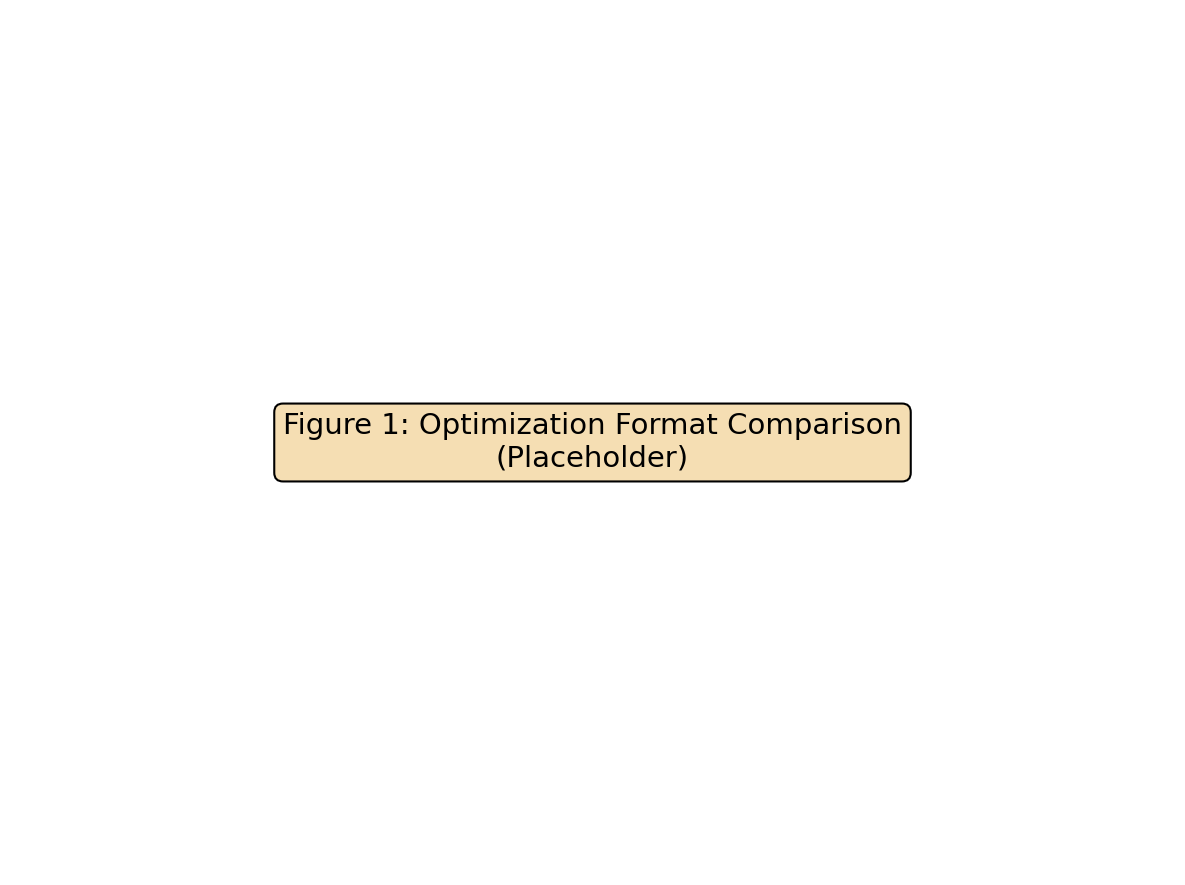
\includegraphics[width=\columnwidth]{fig1_optimization_comparison.png}
\caption{Accuracy-speed trade-offs across optimization formats on Raspberry Pi 4B. ONNX consistently provides the best balance, achieving highest FPS with minimal accuracy degradation. TFLite offers smallest model size but with 1.5--2\% mAP@50 loss due to INT8 quantization.}
\label{fig:optimization_comparison}
\end{figure}

Table~\ref{tab:optimization_format} quantifies the performance differences across optimization formats, normalized to PyTorch baseline.

\begin{table}[!t]
\caption{Optimization Format Performance Comparison (Relative to PyTorch Baseline)}
\label{tab:optimization_format}
\centering
\resizebox{\columnwidth}{!}{
\begin{tabular}{lcccc}
\toprule
\textbf{Format} & \textbf{Speedup} & \textbf{Model Size} & \textbf{RAM Usage} & \textbf{mAP@50} \\
 & \textbf{(×)} & \textbf{Reduction (\%)} & \textbf{Reduction (\%)} & \textbf{Retention (\%)} \\
\midrule
PyTorch & 1.0× & 0\% & 0\% & 100\% \\
ONNX & 1.85× & 3.1\% & 36.7\% & 99.7\% \\
TFLite & 1.52× & 51.6\% & 43.9\% & 97.8\% \\
OpenVINO & 1.76× & 6.3\% & 41.8\% & 99.6\% \\
\bottomrule
\end{tabular}
}
\end{table}

\textbf{Analysis}:

\begin{itemize}
\item \textbf{ONNX Dominates for Edge Deployment}: ONNX achieves 1.85$\times$ average speedup with 99.7\% accuracy retention and 36.7\% RAM reduction, making it the optimal choice for Raspberry Pi deployment. ONNX Runtime's graph optimizations (operator fusion, constant folding, layout optimization) and efficient memory management contribute to this performance advantage.

\item \textbf{TFLite for Storage-Constrained Scenarios}: TFLite's 51.6\% model size reduction makes it attractive for storage-constrained devices or applications requiring model distribution over limited bandwidth. However, the 2.2\% accuracy loss from INT8 quantization may be unacceptable for high-precision applications.

\item \textbf{OpenVINO as Intel-Optimized Alternative}: OpenVINO achieves 1.76$\times$ speedup with 99.6\% accuracy retention, leveraging Intel CPU optimizations (AVX2, VNNI instructions). While slightly slower than ONNX on Raspberry Pi's ARM CPU, OpenVINO may outperform on Intel-based edge devices (e.g., Intel NUC, UP Board).

\item \textbf{Quantization Trade-offs}: TFLite's INT8 quantization reduces model size and memory footprint but introduces quantization errors that disproportionately affect small object detection (disease lesions), explaining the 2.2\% mAP@50 degradation. Quantization-aware training (QAT) could potentially mitigate this accuracy loss \cite{43}.
\end{itemize}

\subsection{Model Architecture Comparison}

Figure~\ref{fig:model_comparison} compares the accuracy-speed trade-offs across YOLO architectures for nano and small variants with ONNX optimization (best-performing format).

\begin{figure}[!t]
\centering
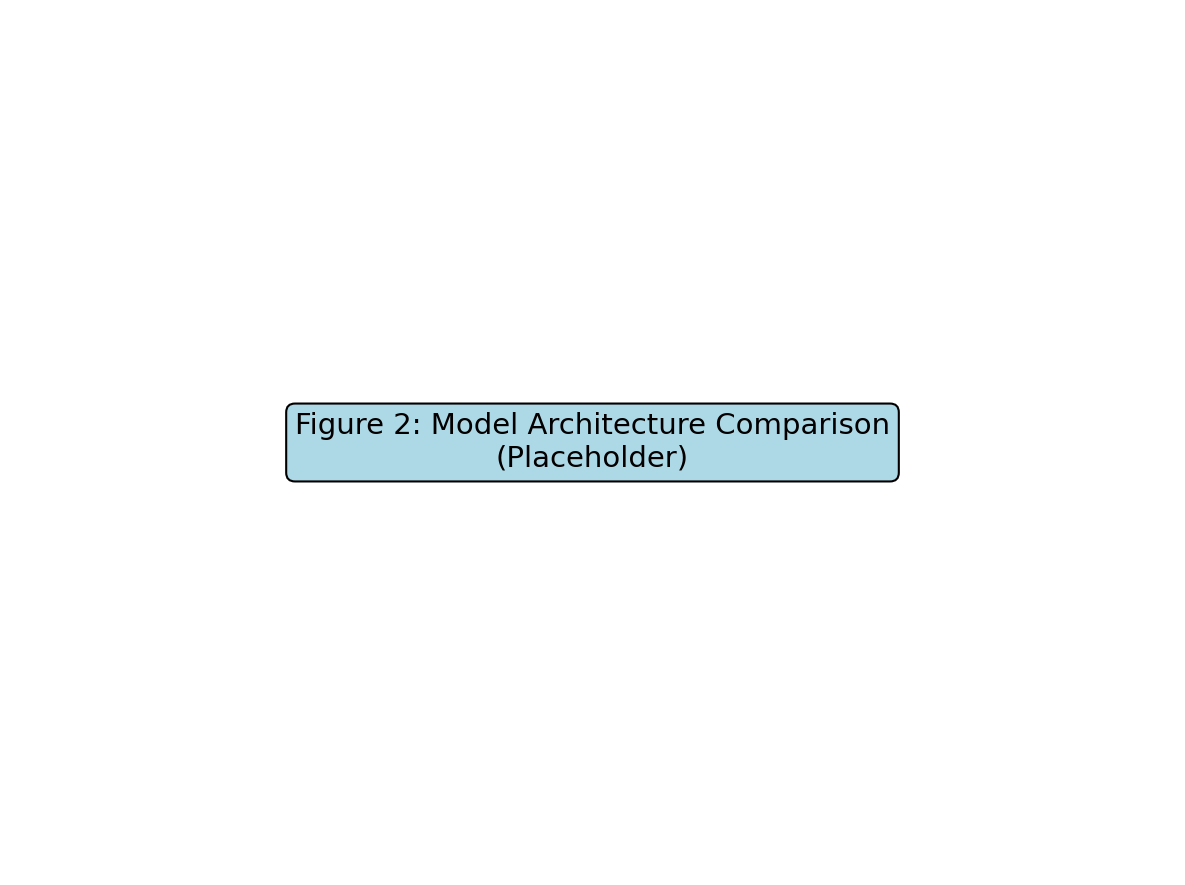
\includegraphics[width=\columnwidth]{fig2_model_comparison.png}
\caption{Accuracy-speed trade-offs across YOLO architectures (nano and small variants) with ONNX optimization on Raspberry Pi 4B. YOLOv11n achieves optimal balance (87.1\% mAP@50, 13.2 FPS), while YOLOv11s provides highest accuracy (89.9\% mAP@50) at reduced speed (6.6 FPS).}
\label{fig:model_comparison}
\end{figure}

\textbf{Comparative Analysis}:

\begin{itemize}
\item \textbf{YOLOv11n: Optimal Balance}: YOLOv11n-ONNX achieves 87.1\% mAP@50 at 13.2 FPS, representing the best accuracy-speed trade-off for real-time edge deployment. This configuration provides sufficient accuracy for practical disease detection while maintaining comfortable real-time performance.

\item \textbf{YOLOv10n: Speed Champion}: YOLOv10n-ONNX achieves the highest FPS (13.8) but with slightly lower accuracy (85.6\% mAP@50). This makes YOLOv10n suitable for applications prioritizing speed over accuracy, such as rapid field surveys or high-throughput screening.

\item \textbf{YOLOv11s: Accuracy Leader}: YOLOv11s-ONNX achieves the highest accuracy (89.9\% mAP@50) but at reduced speed (6.6 FPS), falling below the 10 FPS real-time threshold. This configuration is appropriate for offline analysis or scenarios where accuracy is paramount and real-time performance is not required.

\item \textbf{YOLOv8 and YOLOv12: Competitive Alternatives}: YOLOv8n and YOLOv12n show competitive performance (86.2\% and 86.7\% mAP@50, 12.7 and 12.9 FPS), providing viable alternatives to YOLOv11n with marginal trade-offs in accuracy or speed.

\item \textbf{Architectural Efficiency}: YOLOv11's refined C3k2 blocks and improved attention mechanisms provide measurable advantages in accuracy without sacrificing inference speed, validating the effectiveness of recent architectural innovations \cite{4}, \cite{25}.
\end{itemize}

\subsection{Per-Class Performance Analysis}

Table~\ref{tab:per_class} presents per-class Average Precision (AP@50) for representative models, revealing class-specific detection challenges.

\begin{table}[!t]
\caption{Per-Class Average Precision (AP@50) for Representative Models}
\label{tab:per_class}
\centering
\resizebox{\columnwidth}{!}{
\begin{tabular}{lcccc}
\toprule
\textbf{Model} & \textbf{Algal Leaf} & \textbf{Leaf Blight} & \textbf{Leaf Spot} & \textbf{Healthy} \\
 & \textbf{Spot (\%)} & \textbf{(\%)} & \textbf{(\%)} & \textbf{(\%)} \\
\midrule
YOLOv8n-ONNX & 84.2 & 89.7 & 82.1 & 89.8 \\
YOLOv10n-ONNX & 83.5 & 88.9 & 81.3 & 88.7 \\
YOLOv11n-ONNX & 85.3 & 90.6 & 83.8 & 89.9 \\
YOLOv12n-ONNX & 84.7 & 89.8 & 82.9 & 89.4 \\
YOLOv8s-ONNX & 87.6 & 92.3 & 86.2 & 91.5 \\
YOLOv11s-ONNX & 88.4 & 93.1 & 87.5 & 92.0 \\
\bottomrule
\end{tabular}
}
\end{table}

\textbf{Observations}:

\begin{itemize}
\item \textbf{Leaf Blight: Easiest to Detect}: Leaf Blight achieves the highest AP@50 (88.9--93.1\%) across all models, attributed to its large, distinctive lesions with high contrast against healthy tissue. The water-soaked appearance and irregular shape provide strong visual cues for detection.

\item \textbf{Leaf Spot: Most Challenging}: Leaf Spot exhibits the lowest AP@50 (81.3--87.5\%), reflecting the difficulty of detecting small (1--5 mm), low-contrast lesions that may be confused with natural leaf variations, insect damage, or environmental stress symptoms.

\item \textbf{Algal Leaf Spot: Moderate Difficulty}: Algal Leaf Spot achieves intermediate AP@50 (83.5--88.4\%), with detection challenges arising from variable lesion appearance (color, texture, size) depending on infection stage and environmental conditions.

\item \textbf{Healthy Class: High Precision}: The Healthy class achieves high AP@50 (88.7--92.0\%), indicating reliable discrimination between diseased and healthy leaves. However, false positives may occur when healthy leaves exhibit natural senescence, nutrient deficiencies, or mechanical damage.

\item \textbf{Small Model Advantage}: Small models (YOLOv8s, YOLOv11s) show consistent 3--5\% AP@50 improvement across all classes compared to nano models, with the largest gains for challenging classes (Leaf Spot), demonstrating the value of increased model capacity for difficult detection tasks.
\end{itemize}

\subsection{Practical Deployment Considerations}

Based on our comprehensive evaluation, we provide the following practical recommendations for deploying YOLO-based durian disease detection systems on Raspberry Pi:

\textbf{Recommended Configuration}:
\begin{itemize}
\item \textbf{Model}: YOLOv11n-ONNX (87.1\% mAP@50, 13.2 FPS, 5.0 MB, 318 MB RAM)
\item \textbf{Rationale}: Optimal balance between accuracy, speed, and resource efficiency for real-time edge deployment. Achieves comfortable real-time performance ($>$10 FPS) with sufficient accuracy for practical disease detection.
\item \textbf{Use Cases}: Automated field monitoring, real-time disease alerts, mobile diagnostic tools, IoT-based precision agriculture systems.
\end{itemize}

\textbf{Alternative Configurations}:

\begin{enumerate}
\item \textbf{Speed-Prioritized}: YOLOv10n-ONNX (85.6\% mAP@50, 13.8 FPS)
   \begin{itemize}
   \item For applications requiring maximum throughput (rapid field surveys, high-resolution image scanning).
   \item Trade-off: 1.5\% lower accuracy for 0.6 FPS gain.
   \end{itemize}

\item \textbf{Accuracy-Prioritized}: YOLOv11s-ONNX (89.9\% mAP@50, 6.6 FPS)
   \begin{itemize}
   \item For offline analysis, research applications, or scenarios where accuracy is paramount.
   \item Trade-off: 2.8\% higher accuracy but 50\% slower, below real-time threshold.
   \end{itemize}

\item \textbf{Storage-Constrained}: YOLOv11n-TFLite (85.6\% mAP@50, 10.8 FPS, 2.6 MB)
   \begin{itemize}
   \item For devices with limited storage or bandwidth-constrained model distribution.
   \item Trade-off: 1.5\% lower accuracy and 2.4 FPS slower than ONNX, but 48\% smaller model size.
   \end{itemize}
\end{enumerate}

\textbf{System Integration Guidelines}:

\begin{itemize}
\item \textbf{Image Acquisition}: Use 1920$\times$1080 or 2560$\times$1440 resolution cameras to balance image quality and processing overhead. Higher resolutions (4K) provide better small lesion detection but increase preprocessing time.

\item \textbf{Preprocessing Pipeline}: Implement efficient image resizing (640$\times$640) using OpenCV with INTER\_LINEAR interpolation. Consider hardware-accelerated JPEG decoding on Raspberry Pi 4B's VideoCore VI GPU.

\item \textbf{Batch Processing}: For non-real-time applications, batch multiple images to amortize model loading overhead and improve throughput.

\item \textbf{Power Management}: Implement dynamic frequency scaling and thermal throttling monitoring to prevent performance degradation during extended operation in field conditions.

\item \textbf{Result Post-Processing}: Apply confidence thresholding (0.25--0.35) and Non-Maximum Suppression (NMS, IoU threshold 0.45) to filter false positives and overlapping detections.

\item \textbf{Cloud Integration}: For hybrid edge-cloud architectures, transmit only high-confidence detections or flagged images to cloud for expert review, reducing bandwidth requirements.
\end{itemize}

\textbf{Limitations and Considerations}:

\begin{itemize}
\item \textbf{Environmental Variability}: Model performance may degrade under extreme lighting conditions (direct sunlight, deep shade), motion blur, or occlusion. Consider multi-frame aggregation or active illumination for challenging scenarios.

\item \textbf{Disease Stage Sensitivity}: Early-stage disease symptoms (small, faint lesions) are more difficult to detect than advanced stages. Regular monitoring and low confidence thresholds can improve early detection at the cost of increased false positives.

\item \textbf{Generalization to New Varieties}: Models trained on specific durian varieties may require fine-tuning or domain adaptation for deployment in orchards with different cultivars (Monthong, Musang King, D24).

\item \textbf{Hardware Limitations}: Raspberry Pi 4B's ARM Cortex-A72 CPU limits inference speed compared to specialized AI accelerators (Google Coral TPU, Intel Neural Compute Stick). For applications requiring higher throughput, consider upgrading to Raspberry Pi 5 or alternative edge platforms.

\item \textbf{Seasonal and Geographic Variations}: Disease prevalence, symptom appearance, and environmental conditions vary across seasons and geographic regions. Periodic model retraining or online learning may be necessary for long-term deployment.
\end{itemize}
